

The model used in this project is {\fontfamily{qcr}\selectfont Davlan/bert-base-multilingual-cased-ner-hrl} an NER model for 10 high-resourced languages trained to recognize three types of entities: location (LOC), organizations (ORG), and person (PER). To produce this model, a {\fontfamily{qcr}\selectfont bert-base-multilingual-cased} model was fine-tuned on an aggregation of 10 high-resourced languages \cite{noauthor_bert-base-multilingual-cased_nodate}. The {\fontfamily{qcr}\selectfont cased} part of the model name means the model distinguishes between uppercase and lowercase characters.

Table \ref{tab:NER-output} shows the named entities extracted from the sentence \textit{My name is Elizaveta. I'm from Aberdeen and I study at the University of St Andrews.}

\begin{table}[ht]
  \centering
  \begin{tabular}{|c|c|c|c|c|}
    \hline
    \textbf{entity group} & \textbf{score} & \textbf{word} & \textbf{start} & \textbf{end} \\
    \hline{}
    
    PER  &  0.9997233  &  Elizaveta  &  11  &  20  \\
    LOC  &  0.9991941  &  Aberdeen  &  31  &  39  \\
    ORG  &  0.9998053  &  University of St Andrews  &  59  &  83  \\
    \hline
  \end{tabular}
  \caption{NER Output}
  \label{tab:NER-output}
\end{table}

BERT is a special neural network architecture. It is helpful to understand BERT's predecessors to understand the power of this language model.

\subsection{The Dark Ages of NLP}

Before the NLP Revolution in 2017 (see Section \ref{the-og-transformer}), other neural network architectures were used for NLP tasks, such as recurrent neural networks (RNNs) and convolutional neural networks (CNNs).

RNNs were widely used for NLP tasks because they can process sequential data naturally. One of the significant limitations of RNNs is the vanishing gradient problem, which hinders the model's ability to grasp long-term dependencies in the input sequence. Variants of RNNs (LSTM and GRUs) addressed this problem, allowing the models to handle long-term dependencies in the input sequence. \cite{camacho-collados_embeddings_2022}

CNNs were also used for NLP tasks because they are able to capture local patterns and dependencies in the input sequence. However, CNNs are not as effective at capturing long-term dependencies as RNNs. (\cite{camacho-collados_embeddings_2022}), (\cite{geron_hands-machine_2019}).

Overall, these neural network architectures were effective for some NLP tasks. However, they had limitations in handling long text sequences and capturing global and local dependencies in the input sequence. Transformers have emerged as a powerful alternative to these architectures. They are better suited to processing long text sequences and have performed remarkably in various NLP tasks. (\cite{geron_hands-machine_2019})

\subsection{The OG Transformer} \label{the-og-transformer}

The transformer architecture introduced in "Attention Is All You Need" was a revolutionary advancement in NLP because it provided an alternative to RNNs and CNNs. \cite{vaswani_attention_2017}

One key innovation of the transformer architecture was the attention mechanism. The main idea behind the attention mechanism is that the model can focus on the relevant parts of the input sequence. The transformer would focus on the words \textit{cute} and \textit{hide} to determine the meaning of the word \textit{duck} rather than relying on context windows or sequential processing. This feature of transformers made it possible to capture longer-range dependencies and handle variable-length input sequences better. (\cite{vaswani_attention_2017})

The transformer architecture was also more parallelizable than RNNs and CNNs, making training and inference more efficient. All the words in a sentence are processed simultaneously instead of relying on a previous output to generate the following output. The transformer model could be trained on large-scale datasets in days, compared to the weeks or months it would take to train traditional NLP models. (\cite{vaswani_attention_2017})

RNNs excelled at sequences, while CNNs shined in their ability to extract local features and capture dependencies. Both encode the order and position of words naturally. Transformers took a different approach by using positional encoding, which allowed the models to capture the positional information of words. (\cite{vaswani_attention_2017})

A common problem in deep learning training is the gradient vanishing problem, with which the transformer's predecessors suffered.
The transformer architecture used residual connections and layer normalization to avoid this problem. (\cite{geron_hands-machine_2019})

\subsection{Types of Transformer Models}

The OG Transformer consists of an encoder and a decoder, each composed of multiple layers of neural networks. The transformer processes an input sequence into an output sequence. The encoder processes the input sequence to produce hidden representations. The decoder attends to these hidden representations to generate an output sequence. (\cite{vaswani_attention_2017})

Since the birth of the transformer architecture, several variants have been introduced, including encoder-only, decoder-only, and encoder-decoder models suited to different NLP tasks. (huggingface.co, n.d.)

Encoder-only models only use the encoder portion of the transformer. These models process the input sequence and generate a contextualized embeddings of the sequence. These representations can be used as input to downstream NLP tasks or the model could be fine-tuned for specific tasks (e.g. NER). Encoders are often \textit{bi-directional}, meaning the model has access to left and right contexts. \cite{tunstall_natural_2022}

Decoder-only models use only the decoder portion of the transformer. These models are trained on tasks like language generation i.e. producing text having been given a prompt sequence. Decoders are \textit{auto-regressive}, meaning they only have access to left context for their next word prediction.
Encoder-decoder models use the encoder and decoder portions of the transformer and are most similar to the original transformer. They perform sequence-to-sequence tasks such as machine translation and summarization. (\cite{tunstall_natural_2022})

\subsection{The Incredible BERT}

BERT stands for "Bidirectional Encoder Representations from Transformers." (\cite{vaswani_attention_2017}):

\begin{description}
   \item[Bidirectional:] BERT is a bidirectional model, which means it is trained to look at both the left and right context of a word in a sentence, as opposed to traditional models that only look at the left or right context (\cite{devlin_bert_2019}). For example, \textit{I saw her duck. It was so cute!} and \textit{I saw her duck down to hide.} Both contain the word \textit{duck} and the first part of the sentence does not help disambiguate the word, so BERT's bidirectional property helps address this.
   \item[Encoder:] BERT is an encoder-based model. (\cite{devlin_bert_2019})
   \item[Representations:] BERT encodes word sequences into vector representations that capture the meaning and context of the text. (\cite{devlin_bert_2019})
   \item[from Transformers:] BERT is a transformer-based neural network model. (\cite{devlin_bert_2019})
\end{description}

BERT was an improvement on the original transformer architecture because of the following features:

\begin{description}
   \item[Pre-training:] The BERT model is a language representation model that can be used for different NLP tasks, unlike the original transformer that was designed for specific sequence-to-sequence tasks (\cite{devlin_bert_2019}). Transfer learning makes BERT adaptable, and it has two stages. First, BERT is pre-trained on a vast collection of text (multilingual BERT is trained on a text corpus from 104 languages with the largest Wikipedias - (huggingface.co, n.d.)). This pre-training step enables BERT to comprehend language, which is why it is versatile. Second, BERT is fine-tuned for specific tasks by adding a task-specific output layer and training it on labeled data, like customer reviews with star ratings (\cite{devlin_bert_2019}). This fine-tuning stage applies BERT's language understanding abilities to the specific task at hand. 
   
   \item[Bidirectional encoding:] The original transformer architecture only processed the input sequence in a forward direction. On the other hand, BERT uses a bidirectional encoding scheme, which allows it to consider both the left and right context of a word when generating its representation. This means that BERT can better understand the meaning of a word in the context of its neighboring words. (\cite{devlin_bert_2019})
   
   \item[Fine-tuning:] The pre-trained BERT model can achieve state-of-the-art performance for various tasks by utilizing transfer learning. Adding a task-specific output layer on top lets the model be easily fine-tuned. As a result, state-of-the-art models can be easily created for a wide range of tasks, with less labeled data and without substantial task-specific architecture modifications. (\cite{devlin_bert_2019})
   
   \item[Larger model size:] BERT was trained on a much larger amount of data than the original transformer and had a much larger model size. Larger model size allowed BERT to capture more complex relationships and dependencies in the input sequence, improving performance on a wide range of NLP tasks. (\cite{devlin_bert_2019})
\end{description}

\subsection{uNERthing Entities}

The model used is one of many BERT-based models. These models consist of two main parts: the model body (BERT) and the task-specific classification head (\cite{tunstall_natural_2022}). This can be seen in \ref{fig:bert-ner-body-head}.

\begin{figure}[h]
    \centering
    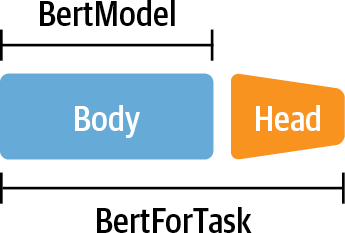
\includegraphics[width=0.2\textwidth]{images/bert-ner-body-head.png}
    \caption{BERT model body \& task-specific classification head (\cite{tunstall_natural_2022})}
    \label{fig:bert-ner-body-head}
\end{figure}

In simple terms, BERT converts sentences into vector representations (called embeddings) that machines can understand. Then the classification head uses this encoded "understanding" to give the words labels LOC, ORG and PER.